\section{Results}
\label{sec:results}

\begin{table*}[t]
\centering
\small
\setlength{\tabcolsep}{4.5pt}
\begin{tabular}{lccccccccccc}
\toprule
 & \multicolumn{1}{c}{Perception} & \multicolumn{3}{c}{Detection} & \multicolumn{4}{c}{Resolution} & \multicolumn{3}{c}{Attribution} \\
\cmidrule(lr){2-2}\cmidrule(lr){3-5}\cmidrule(lr){6-9}\cmidrule(lr){10-12}
Model & Perc. & Flag & FA$\downarrow$ & Det. & Res. & Res.$|$P & ArbF$\downarrow$ & Focus & Span & Input & Strict \\
\midrule
Qwen3-VL-2B & 78.1 & 76.3 & \textbf{16.9} & \textbf{59.4} & 39.4 & 47.4 & 46.6 & 45.5 & 12.3 & 0.0 & 0.0 \\
Qwen3-VL-4B & 83.3 & 94.8 & 37.3 & 57.5 & 41.3 & 47.0 & 51.1 & 76.0 & 87.3 & 1.1 & 0.5 \\
Qwen3-VL-8B & 82.4 & 96.3 & 44.8 & 51.6 & 54.3 & 62.0 & 36.6 & 84.2 & 87.9 & 28.2 & 9.3 \\
Qwen3-VL-30B-A3B & 82.2 & 95.2 & 39.8 & 55.4 & 59.0 & 66.5 & 31.8 & 79.4 & 77.6 & 3.4 & 1.4 \\
Qwen3-VL-32B & \textbf{85.7} & 97.7 & 53.7 & 43.9 & 43.1 & 48.2 & 51.2 & \textbf{86.3} & \textbf{93.3} & 54.2 & \textbf{16.4} \\
\midrule
Qwen2.5-VL-3B & 76.8 & 94.6 & 47.3 & 47.3 & 18.9 & 24.4 & 74.7 & 26.0 & 85.9 & \textbf{67.0} & 10.6 \\
Qwen2.5-VL-7B & 79.5 & \textbf{98.2} & 67.2 & 31.1 & \textbf{65.0} & \textbf{73.4} & \textbf{26.1} & 84.8 & 81.5 & 21.1 & 5.7 \\
Qwen2.5-VL-32B & 82.4 & 93.8 & 43.3 & 50.5 & 48.8 & 56.2 & 41.6 & 80.3 & 82.7 & 10.1 & 2.6 \\
\midrule
InternVL3-2B & 73.6 & 72.0 & 19.9 & 52.1 & 16.9 & 22.7 & 74.6 & 22.4 & 70.8 & 0.0 & 0.0 \\
InternVL3-8B & 82.3 & 93.9 & 35.8 & 58.1 & 49.4 & 55.6 & 42.7 & 72.9 & 11.8 & 3.8 & 1.3 \\
\midrule
SmolVLM2-2.2B & 68.6 & 84.4 & 62.2 & 22.3 & 7.8 & 11.4 & 87.9 & 9.6 & 66.9 & 0.0 & 0.0 \\
\bottomrule
\end{tabular}

\caption{\textbf{Main results} on 1,800 conflicts and 201 controls per model (\%). Perc.: answers from the image with no description. Flag: flags the conflict; FA: flags a faithful control (lower is better); Det.: Flag minus FA. Res.: answers from the image with the description present; Res.$|$P: the same among conflicts the model perceives; ArbF: perceives and flags the conflict yet answers from the text (lower is better); Focus: Res. when told to rely on the image. Span/Input/Strict: attribution report names the edited words / names the text as the wrong input / gets all four fields right. Best in bold. 95\% image-clustered bootstrap intervals are at most $\pm$3.1 points for conflict metrics and $\pm$7.8 points for FA and Det.}
\label{tab:main}
\end{table*}

\subsection{Noticing a conflict is not acting on it}
\label{sec:gap}

Every model reads the description almost perfectly when it is shown alone (text-only accuracy $\geq$99.7\%) and perceives the edited fact from the photo alone on 69--86\% of conflicts (\cref{tab:main}). Detection is high: nine of eleven models flag 84--98\% of conflicts, and the other two 72\% and 76\%. Yet resolution lags far behind, from 8\% (SmolVLM2) to 65\% (Qwen2.5-VL-7B), and conditioning on perception helps only partly: even on conflicts it perceives, the best model answers from the photo on 73\% and the weakest on 11\%.

\Cref{fig:outcomes}a shows the joint outcome per conflict. For six of eleven models the largest outcome is a conflict the model flags but does not answer from the photo, between 33\% and 77\% of conflicts. Arbitration failure isolates this case: among conflicts a model both perceives and flags, it still answers from the text 26\% (Qwen2.5-VL-7B) to 88\% (SmolVLM2) of the time. Noticing and acting are coupled, since resolution is 6--57 points higher on conflicts a model flags than on those it does not, but the coupling is far from complete. Models answer 97--100\% of faithful controls correctly, so the low resolution is specific to conflicts.

\begin{figure*}[t]
\centering
\begin{subfigure}[t]{0.49\linewidth}
\centering
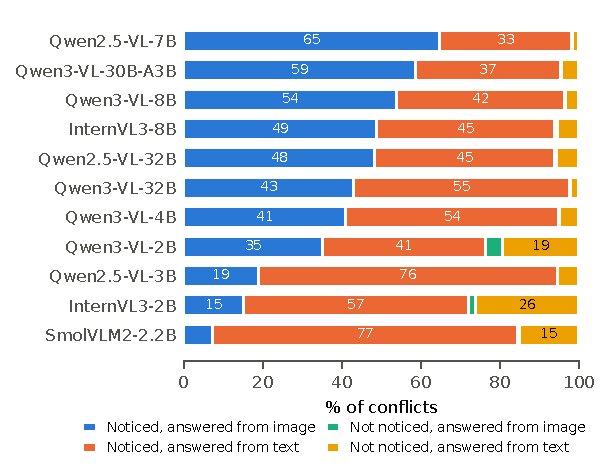
\includegraphics[width=\linewidth]{figures/outcomes.pdf}
\caption{Joint outcome on conflicts, sorted by the noticed-and-resolved share.}
\end{subfigure}\hfill
\begin{subfigure}[t]{0.49\linewidth}
\centering
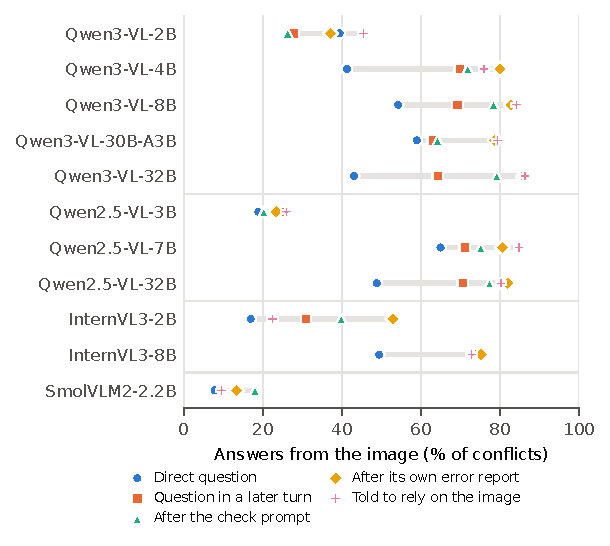
\includegraphics[width=\linewidth]{figures/probes.pdf}
\caption{Answers from the image under each resolution probe.}
\end{subfigure}
\caption{\textbf{Where conflicts go.} (a) ``Noticed'' means the detection probe flags the description; ``answered from image'' means the direct multiple-choice probe picks the photo's answer. (b) Each row shows one model under the direct question, the delayed question, the check prompt, its own error report, and the instruction to rely on the image; the grey bar spans the range.}
\label{fig:outcomes}
\end{figure*}

\subsection{Scale changes the default, not the ability}
\label{sec:scale}

\Cref{fig:scaling} plots three quantities against model size. Answering from the image improves from the 2--4B to the 7--8B models in every family: by 46 points for Qwen2.5-VL (3B to 7B), 32.5 points for InternVL3 (2B to 8B) and 13 points for Qwen3-VL (4B to 8B). Beyond that the trend reverses. Both dense 32B models answer from the image less often than their 7--8B siblings, by 11.2 points for Qwen3-VL [8.9, 13.4] and 16.2 points for Qwen2.5-VL [13.9, 18.6], and the Qwen3-VL 30B-A3B mixture of experts with about 3B active parameters outperforms the dense 32B by 15.9 points (\cref{tab:pairs}; all $p<10^{-10}$, McNemar).

The 32B models are not less able to use the image. They perceive the fact from the photo alone more often than their smaller siblings (86\% and 82\%), and with the instruction to rely on the image they answer from it on 86\% and 80\% of conflicts; the instruction adds 43 points for Qwen3-VL-32B, the largest gain of all models. What changes with scale is the default arbitration between inputs when no instruction is given. A second change is in detection: false alarms on faithful descriptions rise from the 2--3B to the 7--8B model in every family (from 17\% to 45\% for Qwen3-VL), and within Qwen3-VL false-alarm-corrected detection falls from 59\% at 2B to 44\% at 32B. Larger models are more ready to call a description wrong, and less ready to act on it.

\begin{figure*}[t]
\centering
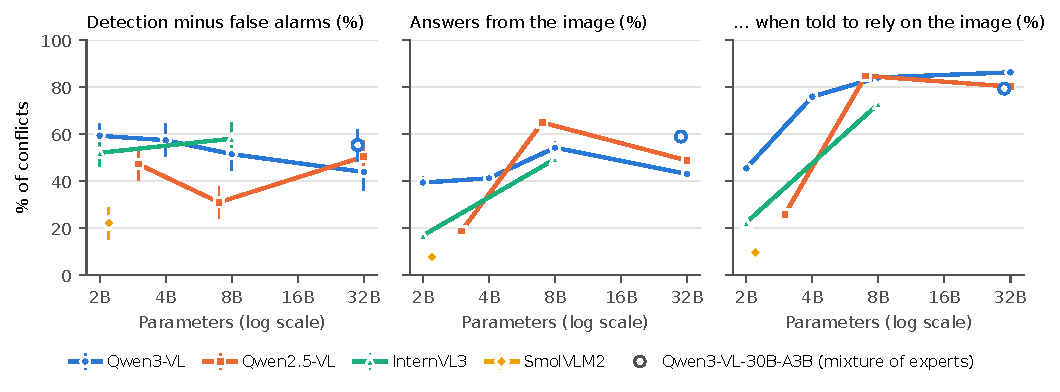
\includegraphics[width=\linewidth]{figures/scaling.pdf}
\caption{\textbf{Scaling within families.} Left: detection minus false alarms. Middle: answers from the image with the description present. Right: the same with an instruction to rely on the image. Hollow marker: Qwen3-VL-30B-A3B (mixture of experts, about 3B active). Bars: 95\% image-clustered bootstrap intervals.}
\label{fig:scaling}
\end{figure*}

\begin{table}[t]
\centering
\scriptsize
\setlength{\tabcolsep}{3pt}
\resizebox{\linewidth}{!}{\begin{tabular}{llccc}
\toprule
Smaller & Larger & $\Delta$ Res. (points) & Discordant (L/S) & $p$ \\
\midrule
Qwen3-VL-2B & Qwen3-VL-4B & +1.8 [$-$0.8, +4.3] & 261/228 & 0.15 \\
Qwen3-VL-4B & Qwen3-VL-8B & +13.0 [+11.0, +15.1] & 325/91 & $<10^{-10}$ \\
Qwen3-VL-8B & Qwen3-VL-32B & $-$11.2 [$-$13.4, $-$8.9] & 125/326 & $<10^{-10}$ \\
Qwen3-VL-8B & Qwen3-VL-30B-A3B & +4.7 [+2.5, +7.0] & 243/158 & $2.6\times10^{-5}$ \\
Qwen3-VL-30B-A3B & Qwen3-VL-32B & $-$15.9 [$-$18.0, $-$13.8] & 82/368 & $<10^{-10}$ \\
Qwen2.5-VL-3B & Qwen2.5-VL-7B & +46.1 [+43.7, +48.4] & 843/13 & $<10^{-10}$ \\
Qwen2.5-VL-7B & Qwen2.5-VL-32B & $-$16.2 [$-$18.6, $-$13.9] & 111/402 & $<10^{-10}$ \\
InternVL3-2B & InternVL3-8B & +32.5 [+29.9, +34.9] & 645/60 & $<10^{-10}$ \\
\bottomrule
\end{tabular}
}
\caption{\textbf{Paired size comparisons} on the same 1,800 conflicts: change in answering from the image (points, 95\% interval), discordant pairs (larger only / smaller only), exact McNemar $p$.}
\label{tab:pairs}
\end{table}

\subsection{What helps: instructions and turn structure}
\label{sec:probes}

An explicit instruction to rely on the image (\cref{fig:outcomes}b) raises resolution by 20--43 points for the seven models of 4B and above, but by only 2--7 points for the four models of 2--3B. Writing an error report and then answering (verbalize) also helps, but its controls show why. For nine of eleven models, merely moving the question to a later turn behind a neutral reply (delay) gains more than the report adds on top of the check control: Qwen3-VL-4B goes from 41\% to 70\% with delay, 72\% with the check prompt and 80\% after its own report. The report itself adds $-$5 to $+$15 points beyond the check control (supplement), and for SmolVLM2 and InternVL3-8B nothing. Putting distance between the misleading text and the question appears to matter more than what the model wrote about it. The open-ended form gives lower resolution than multiple choice for every model above 3B (33--41\% vs.\ 41--65\%), so the gap is not an artefact of the option format.

\subsection{Attribution and self-report consistency}
\label{sec:attribution}

Models are good at pointing at the wrong words: nine of eleven name the edited span in 67--93\% of reports (\cref{tab:main}). They are poor at saying which input is wrong. Only Qwen2.5-VL-3B (67\%) and Qwen3-VL-32B (54\%) usually name the text; the others do so in at most 28\% of reports, and all four fields are right in at most 16\%. More striking, reports often contradict the model's own detection answer. On conflicts it flags in the detection probe, Qwen3-VL-4B writes ``Error: no'' in 99.7\% of its reports, InternVL3-8B in 86\%, Qwen3-VL-2B and Qwen2.5-VL-7B in 71\% and InternVL3-2B in 52\%, while still naming the edited words and the error type in many of them. A model's report of an error is therefore a weak signal of what it has detected. Attribution and resolution are coupled like detection and resolution: ten of eleven models resolve more conflicts when their report names the edited words (by up to 41 points, Qwen2.5-VL-32B).

\subsection{Conflict type and severity}
\label{sec:severity}

Severity grades behave as intended for attributes: pooled over the eleven models, detection falls by 13.3 points [8.1, 18.2] and resolution by 19.0 points [12.7, 25.4] from \Sone to \Sthree. For relations the drops are 4.5 and 9.6 points. Object conflicts are an exception: detection falls by 5.3 points but resolution does not change ($-$0.8 [$-$6.4, 4.7]), and object conflicts are the hardest type to resolve for the four Qwen3-VL models of 4B and above (supplement, per-cell table). Answer position does not explain the results: models pick the photo's answer less often when it is option A (\eg 32\% vs.\ 45--50\% for Qwen3-VL-32B), but correct answers are spread evenly across A--D.
